%%%%%%%%%%%%%%%%%%%%%%%%%%%%%%%%%%%%%%%%%
% Jacobs Portrait Poster
% LaTeX Template
% Version 1.0~gssi01 (04/09/2017)
% (Based on Version 1.0 (29/03/13) of the landscape template
%
% Created by:
% Computational Physics and Biophysics Group, Jacobs University
% https://teamwork.jacobs-university.de:8443/confluence/display/CoPandBiG/LaTeX+Poster
% 
% Further modified by:
% Nathaniel Johnston (nathaniel@njohnston.ca)
%
% Portrait version by:
% John Hammersley
%
% GSSI version by:
% Luca Di Stefano
%
% The landscape version of this template was downloaded from:
% http://www.LaTeXTemplates.com
%
% License:
% CC BY-NC-SA 3.0 (http://creativecommons.org/licenses/by-nc-sa/3.0/)
%
%%%%%%%%%%%%%%%%%%%%%%%%%%%%%%%%%%%%%%%%%

%----------------------------------------------------------------------------------------
%   PACKAGES AND OTHER DOCUMENT CONFIGURATIONS
%----------------------------------------------------------------------------------------

\documentclass[final, 12pt]{beamer}

\usepackage[size=a1, scale=1.15, orientation=portrait]{beamerposter}
% Use the beamerposter package for laying out the poster

\usetheme{gssiposter} % Use the confposter theme supplied with this template

% Define the column widths and overall poster size
% To set effective sepwid, onecolwid and twocolwid values, first choose how many columns you want and how much separation you want between columns
% In this template, the separation width chosen is 0.024 of the paper width and a 4-column layout
% onecolwid should therefore be (1-(# of columns+1)*sepwid)/# of columns e.g. (1-(4+1)*0.024)/4 = 0.22
% Set twocolwid to be (2*onecolwid)+sepwid = 0.464
% Set threecolwid to be (3*onecolwid)+2*sepwid = 0.708

\newlength{\sepwid}
\newlength{\onecolwid}
\newlength{\twocolwid}
\newlength{\threecolwid}
\setlength{\sepwid}{0.02\paperwidth} % Separation width (white space) between columns
\setlength{\onecolwid}{0.28\paperwidth} % Width of one column
\setlength{\twocolwid}{0.56\paperwidth} % Width of two columns
\setlength{\threecolwid}{0.708\paperwidth} % Width of three columns
\setlength{\topmargin}{-0.5in} % Reduce the top margin size

%-----------------------------------------------------------

\usepackage{graphicx}  % Required for including images
\usepackage{booktabs}  % Top and bottom rules for tables

\usepackage{fontawesome}  % Icons in the "contact information" block
\usepackage{microtype}    % Better typesetting

\setbeamertemplate{caption}[numbered]
\usepackage[numbers]{natbib}

\usepackage{multicol}   % Automatic multi-column layout
\usepackage{notoccite}  % Solves problems with citation sorting

\usepackage{fourier}  % Optional: use the Fourier font
\usepackage{caption}  % Optional: subfigures captions
\usepackage{lipsum}   % For "Lorem Ipsum" placeholder text

%----------------------------------------------------------------------------------------
%   TITLE SECTION 
%----------------------------------------------------------------------------------------

\newcommand{\Safesuperscript}[1]{\texorpdfstring{\textsuperscript{#1}}{(#1)}}

%% Insert authors here. Use \Safesuperscript{} for affiliation

\title{Lorem ipsum dolor sit amet consectetuer\protect\\ adipiscing elit}
\author{
  Author One\Safesuperscript{1} \and
  Author Two\Safesuperscript{2}
}

\institute{
  \Safesuperscript{1}Gran Sasso Science Institute (GSSI), L'Aquila, Italy
  \hspace*{3em}
  \Safesuperscript{2}Institute Two, Italy
}

%----------------------------------------------------------------------------------------

\begin{document}

\addtobeamertemplate{block end}{}{\vspace*{2ex}} % White space under blocks
\addtobeamertemplate{block alerted end}{}{\vspace*{2ex}} % White space under highlighted (alert) blocks
\setlength{\belowcaptionskip}{2ex} % White space under figures
\setlength\belowdisplayshortskip{2ex} % White space under equations

\begin{frame}[t] % The whole poster is enclosed in one beamer frame

\begin{columns}[t] % The whole poster consists of three major columns, the second of which is split into two columns twice - the [t] option aligns each column's content to the top

\begin{column}{\onecolwid} % The first column

%----------------------------------------------------------------------------------------
%   ABSTRACT
%----------------------------------------------------------------------------------------

\begin{alertblock}{Abstract}

\lipsum[4]

\end{alertblock}

%----------------------------------------------------------------------------------------
%   INTRODUCTION
%----------------------------------------------------------------------------------------

\begin{block}{Introduction}

\lipsum[2]

\end{block}

\begin{block}{Block Title} Itemize:

\begin{itemize}
    \item Item
    \item Another Item
    \item Yet Another Item
\end{itemize}

\lipsum[3]

\end{block}

%----------------------------------------------------------------------------------------


\begin{column}{\twocolwid}
\begin{figure}
\begin{minipage}{.67\textwidth}
  \centering
  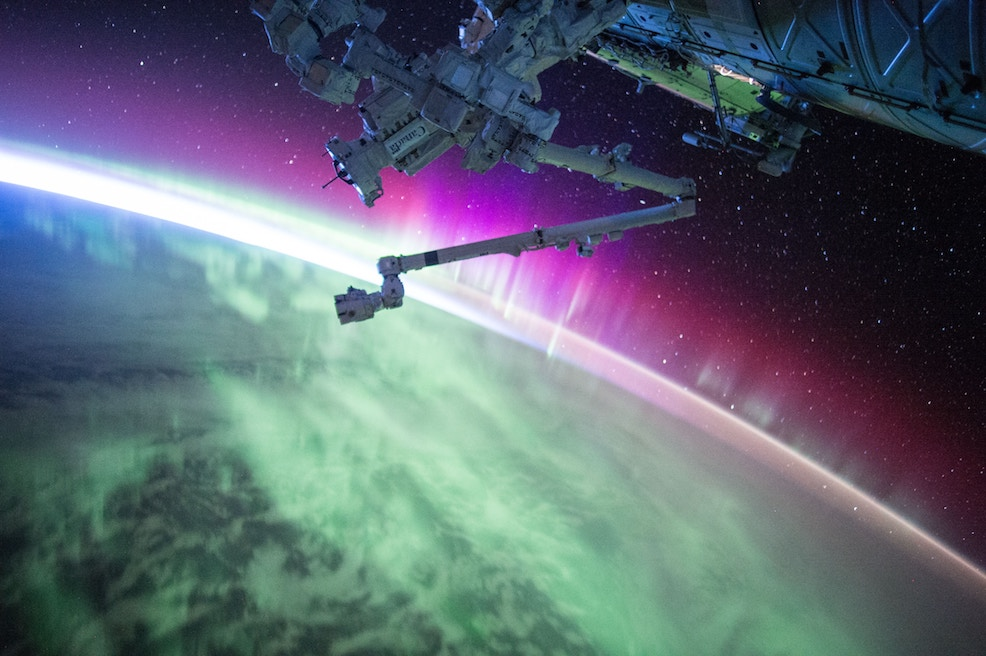
\includegraphics[width=0.95\linewidth]{img/nasa-43567}\hspace*{1.5em}
  \captionof{figure}{Figure caption.}
  \label{fig:fig1}
\end{minipage}\hspace*{1em}%
\begin{minipage}{.45\textwidth}
  \centering
  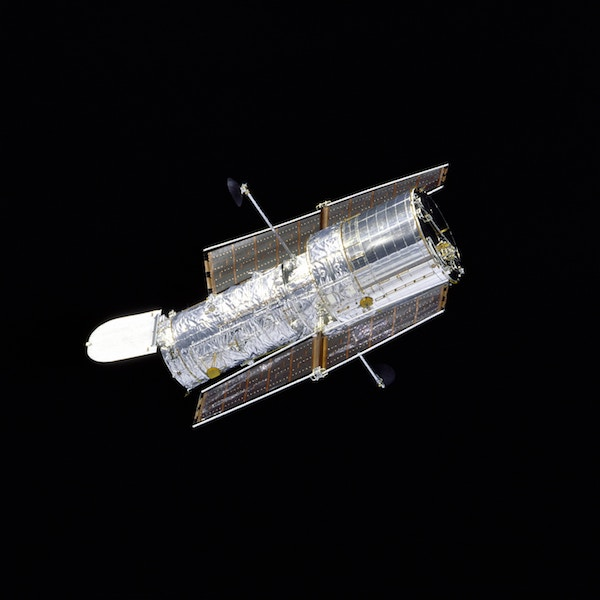
\includegraphics[width=0.95\linewidth]{img/nasa-45070}\hspace*{1.5em}
  \captionof{figure}{Figure caption.}
  \label{fig:fig2}
\end{minipage}
\end{figure}
\end{column}

\end{column} % End of the first column

\begin{column}{\onecolwid} % The second column

%% Use \begin{exampleblock}{} ... \end{exampleblock}
%% to create a block without title.
\begin{exampleblock}{}

\lipsum[2]

\end{exampleblock}

\begin{figure}
\centering
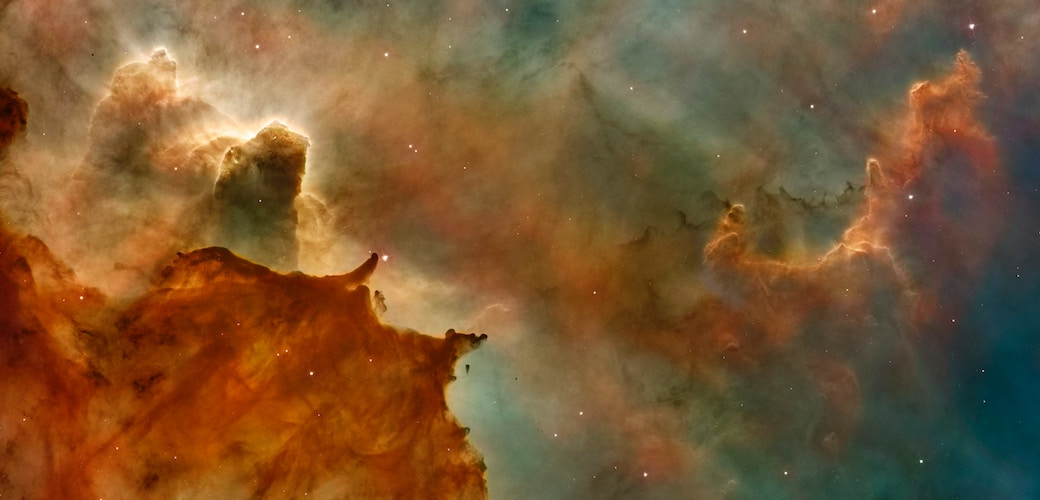
\includegraphics[width=\linewidth]{img/nasa-89127}\hspace*{1.5em}
\caption{Figure caption}
\label{fig:fig3}
\end{figure}

\begin{block}{Block Title}

\lipsum[6-7]

\end{block}

\end{column} % End of the second column

\begin{column}{\onecolwid} % The third column

\begin{block}{Block Title}

\lipsum[1-2]

\end{block}

\begin{figure}
\centering
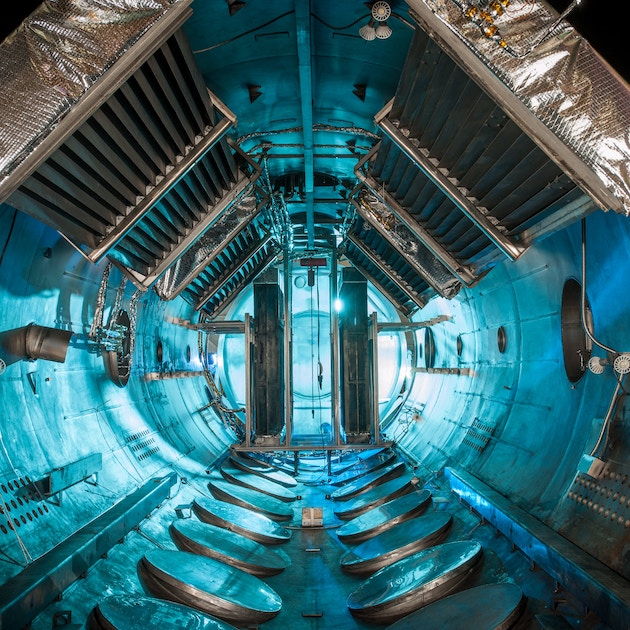
\includegraphics[width=\linewidth]{img/nasa-53885}\hspace*{1.5em}
\caption{Figure caption}
\label{fig:fig4}
\end{figure}

%----------------------------------------------------------------------------------------
%   CONCLUSION
%----------------------------------------------------------------------------------------


\begin{block}{Conclusions and future work}

\lipsum[4]

\end{block}

\end{column} % End of the third column

\end{columns} % End of all the columns in the poster

\hrule

\begin{columns}[t]
\begin{column}{1.5\onecolwid}


%----------------------------------------------------------------------------------------
%   REFERENCES
%----------------------------------------------------------------------------------------

\begin{block}{References}

\begin{multicols}{2}
\small\bibliographystyle{ieeetr}
\nocite{*}
\bibliography{Bibliography}
\end{multicols}

%----------------------------------------------------------------------------------------
%   CONTACT INFORMATION
%----------------------------------------------------------------------------------------


\end{block}
\end{column}
\begin{column}{1.5\onecolwid}  
\begin{block}{Contact Information}
\centering
\begin{multicols}{2}
\small
\begin{itemize}
\item[\faPhoto] \href{https://unsplash.com/@nasa}{Photos: \texttt{unsplash.com/@nasa}}
\item[\faGlobe] \href{http://www.gssi.it/institute/about}{\texttt{gssi.it/institute/about}}
\item[\faEnvelope] \href{mailto:mail1@example.com}{\texttt{mail1@example.com}}
\item[\faEnvelope] \href{mailto:mail2@example.it}{\texttt{mail2@example.com}}
\end{itemize}
\end{multicols}
\end{block}

\begin{center}

\includegraphics[height=2in]{img/gssi.png}\hspace*{1.5em}
%% Insert additional logos here
\end{center}

\end{column}

\end{columns}

\end{frame} % End of the enclosing frame

\end{document}